\documentclass[14pt]{extbook}
\usepackage{multicol, enumerate, enumitem, hyperref, color, soul, setspace, parskip, fancyhdr} %General Packages
\usepackage{amssymb, amsthm, amsmath, latexsym, units, mathtools} %Math Packages
\everymath{\displaystyle} %All math in Display Style
% Packages with additional options
\usepackage[headsep=0.5cm,headheight=12pt, left=1 in,right= 1 in,top= 1 in,bottom= 1 in]{geometry}
\usepackage[usenames,dvipsnames]{xcolor}
\usepackage{dashrule}  % Package to use the command below to create lines between items
\newcommand{\litem}[1]{\item#1\hspace*{-1cm}\rule{\textwidth}{0.4pt}}
\pagestyle{fancy}
\lhead{Progress Quiz 6}
\chead{}
\rhead{Version B}
\lfoot{4563-7456}
\cfoot{}
\rfoot{Summer C 2021}
\begin{document}

\begin{enumerate}
\litem{
Solve the radical equation below. Then, choose the interval(s) that the solution(s) belongs to.\[ \sqrt{-7 x + 8} - \sqrt{4 x + 4} = 0 \]\begin{enumerate}[label=\Alph*.]
\item \( x \in [0.69,2.16] \)
\item \( x_1 \in [-0.38, 0.45] \text{ and } x_2 \in [-1.86,2.14] \)
\item \( x_1 \in [-1.05, -0.37] \text{ and } x_2 \in [-1.86,2.14] \)
\item \( x \in [-0.38,0.45] \)
\item \( \text{All solutions lead to invalid or complex values in the equation.} \)

\end{enumerate} }
\litem{
What is the domain of the function below?\[ f(x) = \sqrt[6]{-3 x + 8} \]\begin{enumerate}[label=\Alph*.]
\item \( [a, \infty), \text{where } a \in [0.8, 5.1] \)
\item \( [a, \infty), \text{where } a \in [-0.1, 0.6] \)
\item \( (-\infty, \infty) \)
\item \( (-\infty, a], \text{where } a \in [-1.6, 2.6] \)
\item \( (-\infty, a], \text{ where } a \in [0.5, 4.4] \)

\end{enumerate} }
\litem{
Solve the radical equation below. Then, choose the interval(s) that the solution(s) belongs to.\[ \sqrt{12 x^2 + 48} - \sqrt{50 x} = 0 \]\begin{enumerate}[label=\Alph*.]
\item \( x \in [2.6,4] \)
\item \( x_1 \in [-5.1, -1.3] \text{ and } x_2 \in [-2.5,-0.5] \)
\item \( x \in [1.2,2.6] \)
\item \( \text{All solutions lead to invalid or complex values in the equation.} \)
\item \( x_1 \in [1.2, 2.6] \text{ and } x_2 \in [0.67,10.67] \)

\end{enumerate} }
\litem{
Choose the graph of the equation below.\[ f(x) = - \sqrt[3]{x + 10} - 4 \]\begin{enumerate}[label=\Alph*.]
\begin{multicols}{2}\item 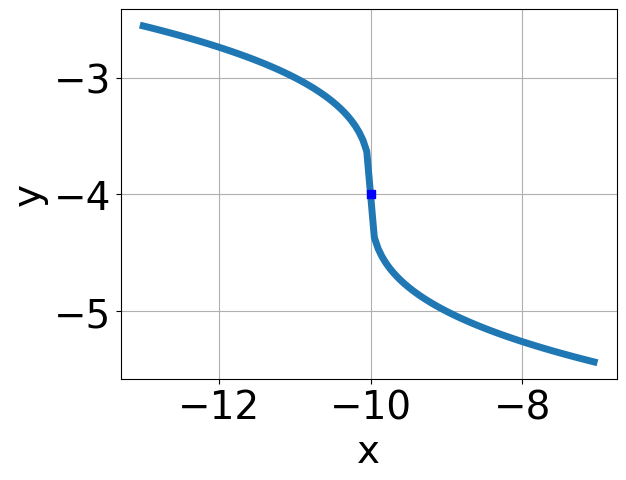
\includegraphics[width = 0.3\textwidth]{../Figures/radicalEquationToGraphAB.png}\item 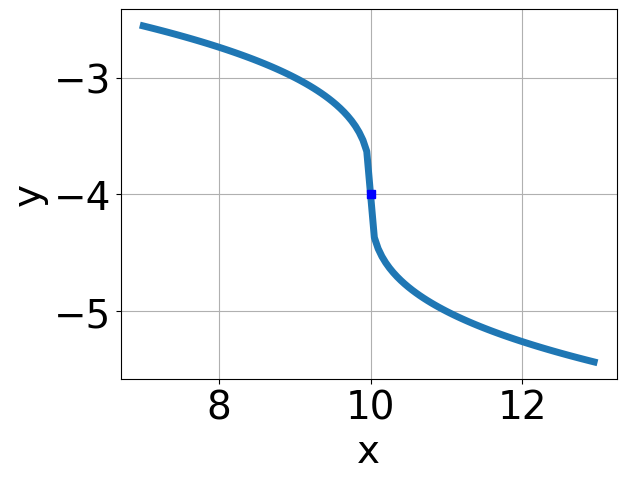
\includegraphics[width = 0.3\textwidth]{../Figures/radicalEquationToGraphBB.png}\item 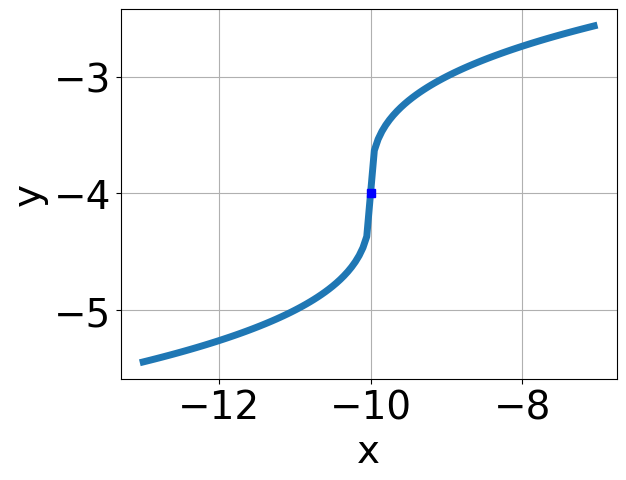
\includegraphics[width = 0.3\textwidth]{../Figures/radicalEquationToGraphCB.png}\item 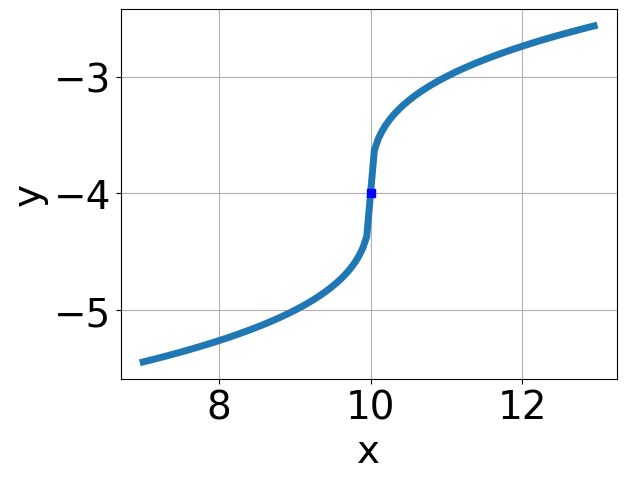
\includegraphics[width = 0.3\textwidth]{../Figures/radicalEquationToGraphDB.png}\end{multicols}\item None of the above.
\end{enumerate} }
\litem{
Solve the radical equation below. Then, choose the interval(s) that the solution(s) belongs to.\[ \sqrt{-18 x^2 - 18} - \sqrt{85 x} = 0 \]\begin{enumerate}[label=\Alph*.]
\item \( x \in [-1.22,0.78] \)
\item \( x_1 \in [2.5, 9.5] \text{ and } x_2 \in [0.13,1.08] \)
\item \( \text{All solutions lead to invalid or complex values in the equation.} \)
\item \( x_1 \in [-5.5, -2.5] \text{ and } x_2 \in [-0.33,-0.17] \)
\item \( x \in [-5.5,-2.5] \)

\end{enumerate} }
\litem{
Choose the equation of the function graphed below.
\begin{center}
    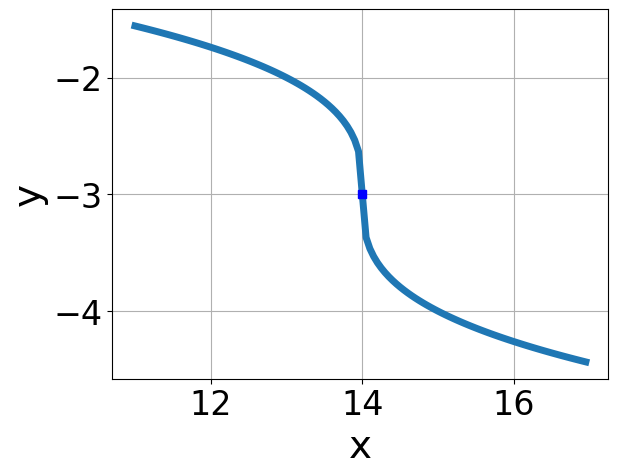
\includegraphics[width=0.5\textwidth]{../Figures/radicalGraphToEquationCopyB.png}
\end{center}
\begin{enumerate}[label=\Alph*.]
\item \( f(x) = \sqrt[3]{x + 14} - 3 \)
\item \( f(x) = \sqrt[3]{x - 14} - 3 \)
\item \( f(x) = - \sqrt[3]{x + 14} - 3 \)
\item \( f(x) = - \sqrt[3]{x - 14} - 3 \)
\item \( \text{None of the above} \)

\end{enumerate} }
\litem{
Choose the graph of the equation below.\[ f(x) = - \sqrt[3]{x - 10} + 5 \]\begin{enumerate}[label=\Alph*.]
\begin{multicols}{2}\item 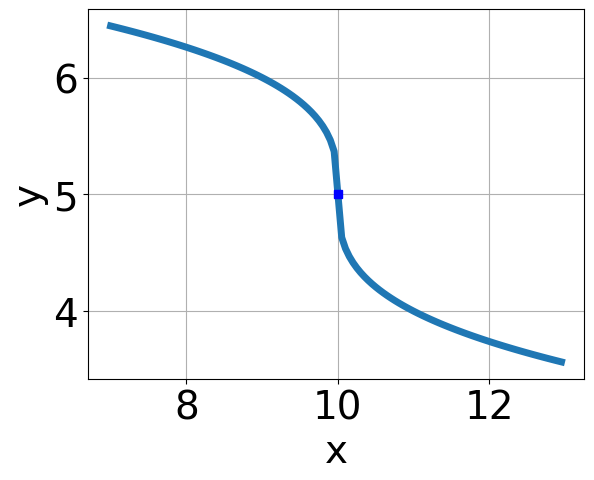
\includegraphics[width = 0.3\textwidth]{../Figures/radicalEquationToGraphCopyAB.png}\item 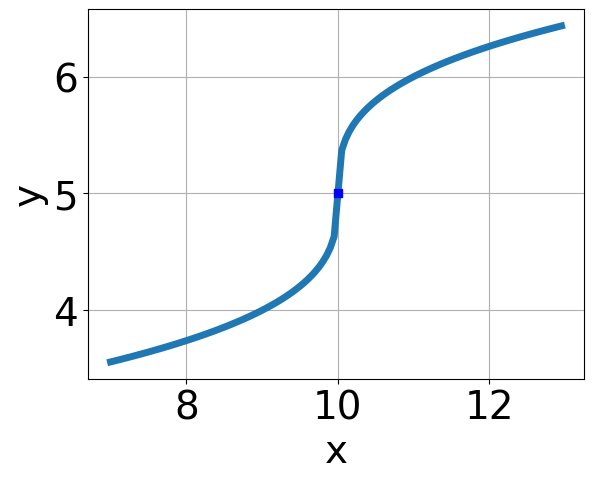
\includegraphics[width = 0.3\textwidth]{../Figures/radicalEquationToGraphCopyBB.png}\item 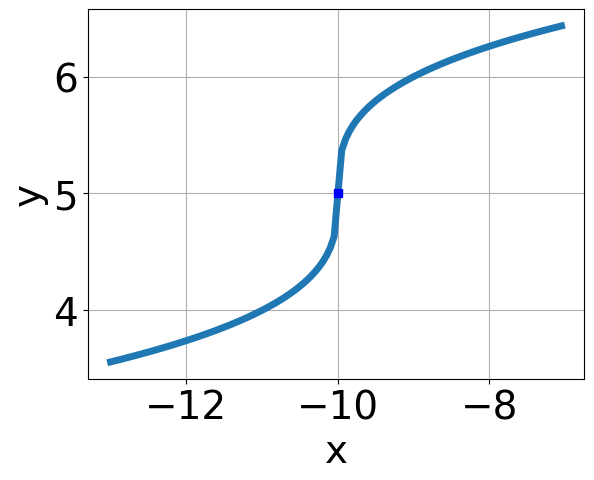
\includegraphics[width = 0.3\textwidth]{../Figures/radicalEquationToGraphCopyCB.png}\item 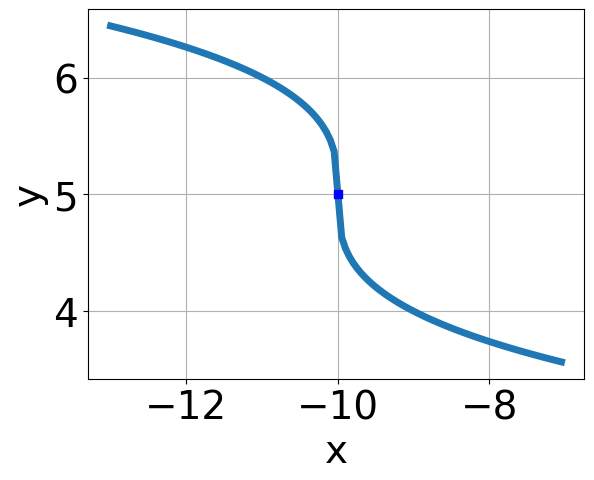
\includegraphics[width = 0.3\textwidth]{../Figures/radicalEquationToGraphCopyDB.png}\end{multicols}\item None of the above.
\end{enumerate} }
\litem{
Choose the equation of the function graphed below.
\begin{center}
    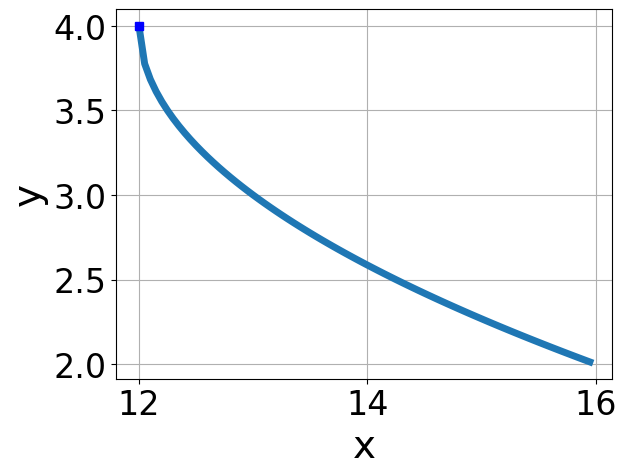
\includegraphics[width=0.5\textwidth]{../Figures/radicalGraphToEquationB.png}
\end{center}
\begin{enumerate}[label=\Alph*.]
\item \( f(x) = \sqrt[3]{x + 12} + 4 \)
\item \( f(x) = \sqrt[3]{x - 12} + 4 \)
\item \( f(x) = - \sqrt[3]{x + 12} + 4 \)
\item \( f(x) = - \sqrt[3]{x - 12} + 4 \)
\item \( \text{None of the above} \)

\end{enumerate} }
\litem{
What is the domain of the function below?\[ f(x) = \sqrt[3]{7 x + 6} \]\begin{enumerate}[label=\Alph*.]
\item \( \text{The domain is } [a, \infty), \text{   where } a \in [-1.06, -0.52] \)
\item \( (-\infty, \infty) \)
\item \( \text{The domain is } (-\infty, a], \text{   where } a \in [-1.11, 0.26] \)
\item \( \text{The domain is } [a, \infty), \text{   where } a \in [-1.29, -1.11] \)
\item \( \text{The domain is } (-\infty, a], \text{   where } a \in [-2.33, -0.99] \)

\end{enumerate} }
\litem{
Solve the radical equation below. Then, choose the interval(s) that the solution(s) belongs to.\[ \sqrt{9 x + 6} - \sqrt{-2 x + 9} = 0 \]\begin{enumerate}[label=\Alph*.]
\item \( x \in [-0.29,0.79] \)
\item \( \text{All solutions lead to invalid or complex values in the equation.} \)
\item \( x_1 \in [-0.99, -0.24] \text{ and } x_2 \in [-4.73,1.27] \)
\item \( x \in [-1.41,-1.07] \)
\item \( x_1 \in [-0.99, -0.24] \text{ and } x_2 \in [4.5,5.5] \)

\end{enumerate} }
\end{enumerate}

\end{document}